\section{Векторы}
\index{Векторы!компланарные} Векторы называются \textbf{компланарными}, если они лежат в одной плоскости.

Некомпланарные векторы $\overline a, \overline b, \overline c$, начала которых находятся в одной точке, называются \textbf{правой тройкой~$(\overline a, \overline b, \overline c)$}, если с конца~$\overline c$ кратчайший поворот от~$\overline a$ к~$\overline b$ виден против часовой стрелки при условии, иначе~--- \textbf{левой тройкой~$(\overline a, \overline b, \overline c)$}.
Также говорят о \textbf{левой} или \textbf{правой ориентации тройки}.

\subsection{Векторное произведение}
\index{Произведение!векторное} Векторным произведением векторов $\overline a$ и $\overline b$ называется вектор~$\overline c$ такой, что:
\begin{itemize}
	\item $|\overline c| = |\overline a| \cdot |\overline b| \cdot \sin \angle(\overline a, \overline b)$
	\item $\overline c \perp \overline a \lAnd \overline c \perp \overline b$
	\item $(\overline a, \overline b, \overline c)$~--- правая тройка
\end{itemize}
и обозначается $[\overline a \cdot \overline b]$ или $[\overline a\,\overline b]$.

Свойства векторного произведения:
\begin{enumerate}
	\item $[\overline a\,\overline a] = \overline 0$
	\begin{proof}
	\begin{equation*}
	\angle(\overline a, \overline a) = 0 \Rightarrow
	|[\overline a\,\overline a]| = |\overline a|^2 \cdot \sin \angle(\overline a, \overline a) = 0 \Rightarrow
	[\overline a\,\overline a] = \overline 0
	\end{equation*}
	\end{proof}
	
	\item $[\overline a\,\overline b] = -[\overline b\,\overline a]$
	\begin{proof}
	Достаточно заметить, что тройки $(\overline a, \overline b, \overline c)$ и $(\overline b, \overline a, \overline c)$ имеют разную ориентацию.
	\end{proof}
	
	\item $\forall \alpha \in \mathbb R \ [(\alpha \overline a)\,\overline b] = \alpha [\overline a\,\overline b]$
	\begin{proof}
	\begin{enumerate}
		\item Пусть $\alpha < 0$, тогда $[(\alpha \overline a)\,\overline b] = -|\alpha| [\overline a\,\overline b] = \alpha [\overline a\,\overline b]$.
		\item Пусть $\alpha \geqslant 0$, тогда $[(\alpha \overline a)\,\overline b] = |\alpha| [\overline a\,\overline b] = \alpha [\overline a\,\overline b]$.
	\end{enumerate}
	\end{proof}
	
	\item $[(\overline a + \overline b)\,\overline c] = [\overline a\,\overline c] + [\overline b\,\overline c]$
	\begin{proof}
	\begin{enumerate}
		\item Пусть $\overline a, \overline b, \overline c$ лежат в плоскости~$\pi$.
		Введём векторы $\overline e \colon \overline e \in \pi \lAnd \overline e \perp \overline c$ и $\overline g$ такой, что:
		\begin{itemize}
			\item $[\overline a\,\overline c] = |\overline a| \cdot |\overline c| \cdot \sin \angle(\overline a, \overline c) \cdot \overline g$
			\item $[\overline b\,\overline c] = |\overline b| \cdot |\overline c| \cdot \sin \angle(\overline b, \overline c) \cdot \overline g$
		\end{itemize}
		
		Тогда
		\begin{equation*}
		[\overline a\,\overline c] = 
		|\overline a| \cdot |\overline c| \cdot \cos \angle(\overline a, \overline e) \cdot \overline g =
		\pr_{\overline e} \overline a \cdot |\overline c| \cdot \overline g
		\end{equation*}
		\begin{equation*}
		[\overline b\,\overline c] = 
		|\overline b| \cdot |\overline c| \cdot \cos \angle(\overline b, \overline e) \cdot \overline g =
		\pr_{\overline e} \overline a \cdot |\overline c| \cdot \overline g
		\end{equation*}
		\begin{equation*}
		[(\overline a + \overline b)\,\overline c] =
		\pr_{\overline e} (\overline a + \overline b) \cdot |\overline c| \cdot \overline g =
		\pr_{\overline e} \overline a \cdot |\overline c| \cdot \overline g +
		\pr_{\overline e} \overline b \cdot |\overline c| \cdot \overline g =
		[\overline a\,\overline c] + [\overline b\,\overline c]
		\end{equation*}
		
		\item Пусть $\overline a, \overline b, \overline c$ некомпланарны, тогда $[(\overline a + \overline b)\,\overline c], [\overline a\,\overline c], [\overline b\,\overline c] \perp \overline c \Rightarrow
		[(\overline a + \overline b)\,\overline c], [\overline a\,\overline c], [\overline b\,\overline c]$ компланарны $\Rightarrow$
		$\alpha [(\overline a + \overline b)\,\overline c] \opbr=
		\beta [\overline a\,\overline c] \opbr+ \gamma [\overline b\,\overline c]$.
		
		\begin{minipage}[t]{95mm}\noindent
		Докажем, что $\alpha = \beta$.
		\begin{itemize}
			\item $\alpha [(\overline a + \overline b)\,\overline c] =
			\beta [\overline a\,\overline c] + \gamma [\overline b\,\overline c] \Rightarrow
			\alpha (\overline a + \overline b)\,\overline c\,\overline b =
			\beta \overline a\,\overline c\,\overline b$
			
			\item Пусть $V_1$ и $V_2$~--- объёмы параллелепипедов, построенных на $OA$, $OB$, $OH$ и $OC$, $OB$, $OH$ соответственно, тогда $S(OACB) = S(OCDB) \opbr\Rightarrow
			V_1 = V_2 \opbr\Rightarrow
			\overline a\,\overline b\,\overline c = (\overline a + \overline b)\,\overline b\,\overline c \opbr\Rightarrow
			\overline a\,\overline c\,\overline b = (\overline a + \overline b)\,\overline c\,\overline b$
		\end{itemize}
		
		Отсюда $\alpha = \beta$.
		Аналогично $\alpha = \gamma$.
		\end{minipage}
		\hfill
		\begin{minipage}[t]{71mm}\noindent
		\begin{flushright}
		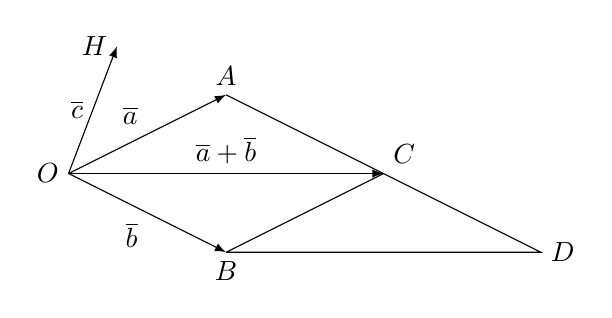
\begin{tikzpicture}[>=latex]
		\draw[->] (0, 0, 0) coordinate (O) node[left] {$O$}
				-- node[above left] {$\overline a$} (2, 1, 0) coordinate (A) node[above] {$A$};
		\draw[->] (O) -- node[below left] {$\overline b$} (2, -1, 0) coordinate (B) node[below] {$B$};
		\draw[->] (O) -- node[above] {$\overline a + \overline b$}
				(4, 0, 0) coordinate (C) node[above right] {$C$};
		\draw (C) -- (A)
			(B) -- (C) -- (6, -1, 0) coordinate (D) node[right] {$D$} -- (B);
		\draw[->] (O) -- node[left] {$\overline c$} (1, 2, 1) coordinate (H) node[left] {$H$};
		\end{tikzpicture}
		\end{flushright}
		\end{minipage}
	\end{enumerate}
	\end{proof}
\end{enumerate}